\documentclass[12pt, letterpaper, twoside]{article}
\usepackage[utf8]{inputenc}
\usepackage{graphicx}
\graphicspath{ {images/} }
 
\title{Covid data visualisation using country_converter}
\author{Rubaba Mammadova \thanks{Memorial University of Newfoundland}}
\date{\today}

\begin{document}
\maketitle
My project focuses on visualisation of covid data via third-party Python package �coco�. �Coco� is country converter library to convert and match country names between different classifications and between different naming versions. 
 \begin{figure}[h]
    \centering
    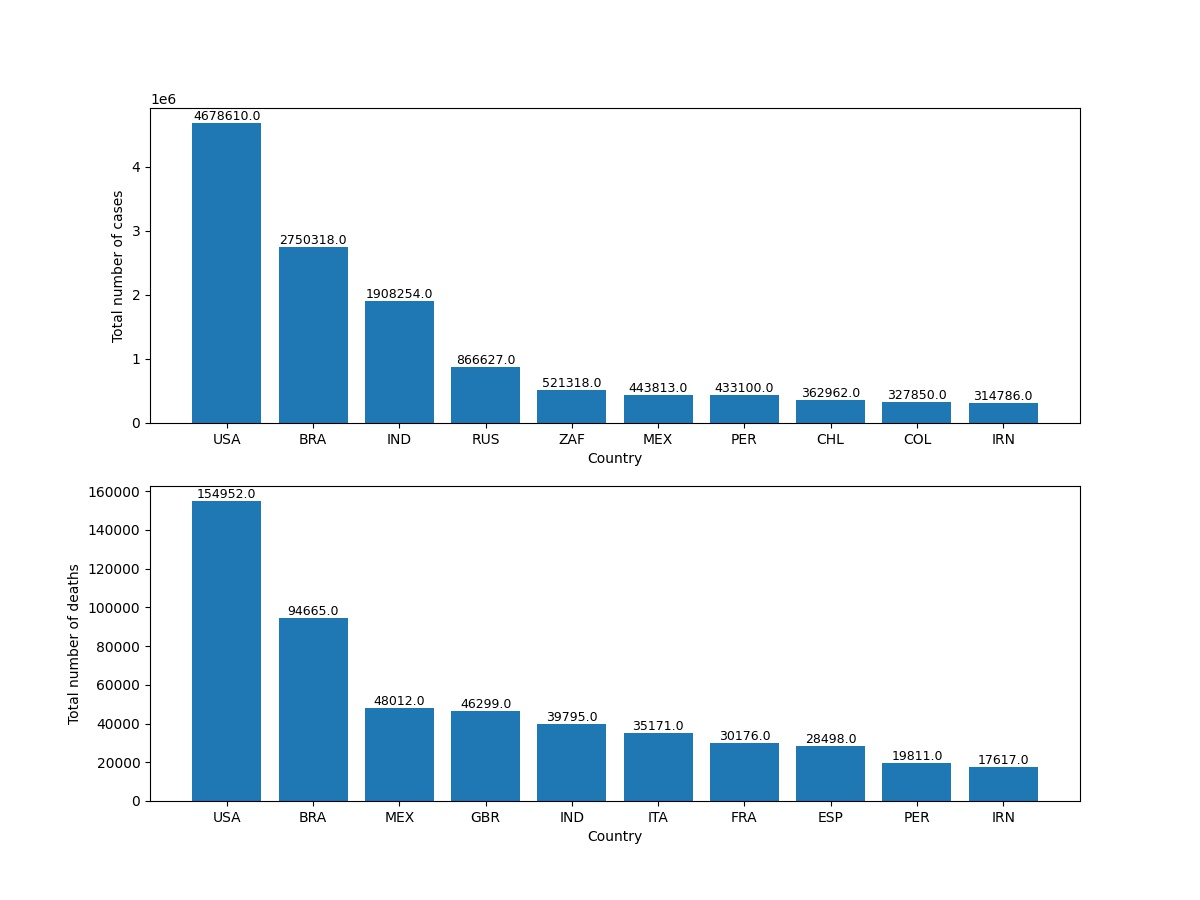
\includegraphics[width=0.25\textwidth]{plot1.jpg}
    \caption{nature}
    \label{fig:myplot1 label}
\end{figure}
 
As you can see in the figure \ref{fig:myplot1 label}, the 
function grows near 0. Also, in the page \pageref{fig:myplot1 label} 
is the same example.
We have now added a title, author and date to our first \LaTeX{} document!
 \begin{figure}[h]
    \centering
    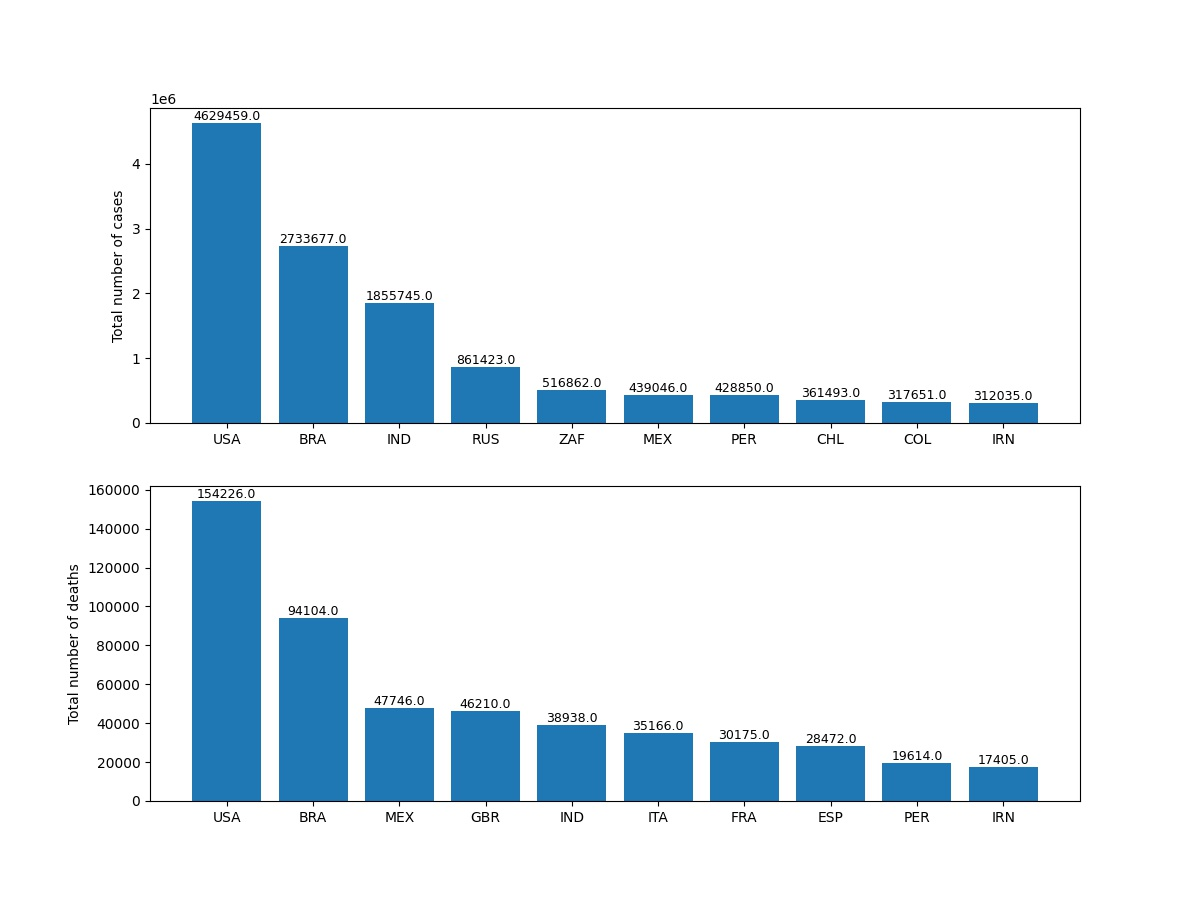
\includegraphics[width=0.25\textwidth]{plot2.jpg}
    \caption{sun}
    \label{fig:sun}
\end{figure}
 
As you can see in the figure \ref{fig:sun}, the 
function grows near 0. Also, in the page \pageref{fig:sun} 
is the same example.

\end{document}
